% !TEX program = xelatex
% 人机交互导论 · 课程设计汇报：第三部分《周边旅游》
% 作者：郎若谷 2351871    编译：xelatex（依赖 ctex，Windows 自带宋体/黑体即可）
% 截图放在 ./screenshots/ 下；示意图用 TikZ 矢量绘制。

\documentclass[aspectratio=169,UTF8]{ctexbeamer}

\usepackage{graphicx}
\usepackage{tikz}
\usetikzlibrary{arrows.meta,positioning,calc,shadows}

%==================== 配色（沿用项目与作业的色板）====================
\definecolor{ink}{HTML}{0F172A}
\definecolor{mainblue}{HTML}{2563EB}
\definecolor{softblue}{HTML}{EAF2FF}
\definecolor{mint}{HTML}{DFF7EA}
\definecolor{peach}{HTML}{FFE7C2}
\definecolor{graytext}{HTML}{4B5563}
\definecolor{linegray}{HTML}{CBD5E1}
\definecolor{foodorange}{HTML}{F7943E}
\definecolor{attrgreen}{HTML}{00A040}
\definecolor{accentred}{HTML}{E2231A}

%==================== 主题定制 ====================
\setbeamertemplate{navigation symbols}{}
\setbeamercolor{background canvas}{bg=white}
\setbeamercolor{normal text}{fg=ink}
\setbeamercolor{structure}{fg=mainblue}
\setbeamercolor{frametitle}{fg=ink}
\setbeamerfont{frametitle}{series=\bfseries,size=\Large}
\setbeamercolor{summarybox}{fg=ink,bg=mint}
\usefonttheme{professionalfonts}

% 方块项目符号
\setbeamertemplate{itemize item}{\raisebox{0.2ex}{\color{mainblue}\rule{0.72ex}{0.72ex}}}
\setbeamertemplate{itemize subitem}{\raisebox{0.25ex}{\color{graytext}\rule{0.5ex}{0.5ex}}}

% 标题：左侧蓝色竖条 + 粗体标题 + 蓝转灰的细分割线
\setbeamertemplate{frametitle}{%
  \vskip0.55em%
  \hbox{\hspace{0.25em}{\color{mainblue}\rule[-0.12em]{3.2pt}{1.02em}}\hspace{0.5em}%
    {\usebeamercolor[fg]{frametitle}\usebeamerfont{frametitle}\insertframetitle}}%
  \vskip3pt%
  \hbox{\hspace{0.25em}{\color{mainblue}\rule{2.4cm}{1.6pt}}%
    {\color{linegray}\rule{0.72\paperwidth}{0.55pt}}}%
  \vskip2pt%
}

% 页脚：细线 + 课程 / 作者 / 页码
\setbeamertemplate{footline}{%
  \vskip2pt%
  \hbox to\paperwidth{\hspace{0.7cm}{\color{linegray}\rule{\dimexpr\paperwidth-1.4cm\relax}{0.5pt}}\hspace{0.7cm}}%
  \vskip3pt%
  \hbox to\paperwidth{\hspace{0.7cm}%
    {\scriptsize\color{graytext}人机交互导论\,·\,课程设计}\hfill%
    {\scriptsize\color{graytext}周边旅游\,·\,郎若谷}\hfill%
    {\scriptsize\color{mainblue}\insertframenumber\,/\,6}\hspace{0.7cm}}%
  \vskip6pt%
}

%==================== 自定义命令 ====================
% 图槽：截图带白边圆角与柔和阴影
\newcommand{\shot}[3]{%
  \begin{tikzpicture}
    \node[inner sep=2pt,draw=linegray,line width=0.6pt,rounded corners=5pt,fill=white,
          drop shadow={shadow xshift=0.5pt,shadow yshift=-0.7pt,opacity=0.18}]
      {\includegraphics[width=#1,height=#2,keepaspectratio]{#3}};
  \end{tikzpicture}%
}
\newcommand{\shottrim}[7]{%
  \begin{tikzpicture}
    \node[inner sep=2pt,draw=linegray,line width=0.6pt,rounded corners=5pt,fill=white,
          drop shadow={shadow xshift=0.5pt,shadow yshift=-0.7pt,opacity=0.18}]
      {\includegraphics[width=#1,height=#2,keepaspectratio,trim=#3 #4 #5 #6,clip]{#7}};
  \end{tikzpicture}%
}
% 图注
\newcommand{\imgcap}[1]{\\[3pt]{\scriptsize\color{graytext}#1}}
\newcommand{\tightimgcap}[1]{\\[1pt]{\tiny\color{graytext}#1}}

% 插画卡片：用于无文字图像资产与裁切后的视觉说明
\newcommand{\assetcard}[3]{%
  \begin{tikzpicture}
    \node[inner sep=0pt,draw=linegray,line width=0.6pt,rounded corners=7pt,fill=white,
          drop shadow={shadow xshift=0.6pt,shadow yshift=-0.8pt,opacity=0.16}]
      {\includegraphics[width=#1,height=#2,keepaspectratio]{#3}};
  \end{tikzpicture}%
}

\begin{document}

%==================== 第 1 页：引入 ====================
\begin{frame}{周边旅游：到站之后，去哪儿？}
  \begin{columns}[T,totalwidth=\textwidth]
    \begin{column}{0.50\textwidth}
      \small
      前两部分解决了\textbf{怎么走、票价多少}。走出闸机之后，乘客还会问：附近有什么值得吃、值得看？

      \vskip6pt
      全网 96 个车站、2514 个兴趣点；如果全部铺开，只会造成选择过载。本部分的目标是让陌生站点周边变得\textcolor{mainblue}{\textbf{看得懂、选得快、信得过、走得通}}。

      \vskip9pt
      \begin{tikzpicture}[font=\scriptsize]
        \node[draw=mainblue!30,fill=softblue,rounded corners=5pt,minimum width=1.95cm,minimum height=0.82cm,align=center] at (0,0)
          {{\bfseries 96}\\[-1pt]{\tiny 车站}};
        \node[draw=foodorange!45,fill=foodorange!10,rounded corners=5pt,minimum width=1.95cm,minimum height=0.82cm,align=center] at (2.18,0)
          {{\bfseries 2514}\\[-1pt]{\tiny 兴趣点}};
        \node[draw=attrgreen!35,fill=mint,rounded corners=5pt,minimum width=1.95cm,minimum height=0.82cm,align=center] at (4.36,0)
          {{\bfseries 4 步}\\[-1pt]{\tiny 看选信走}};
      \end{tikzpicture}
    \end{column}
    \begin{column}{0.48\textwidth}
      \centering
      \begin{tikzpicture}
        \node[inner sep=0pt,rounded corners=8pt,
              draw=linegray,line width=0.6pt,
              drop shadow={shadow xshift=0.6pt,shadow yshift=-0.8pt,opacity=0.16}]
          {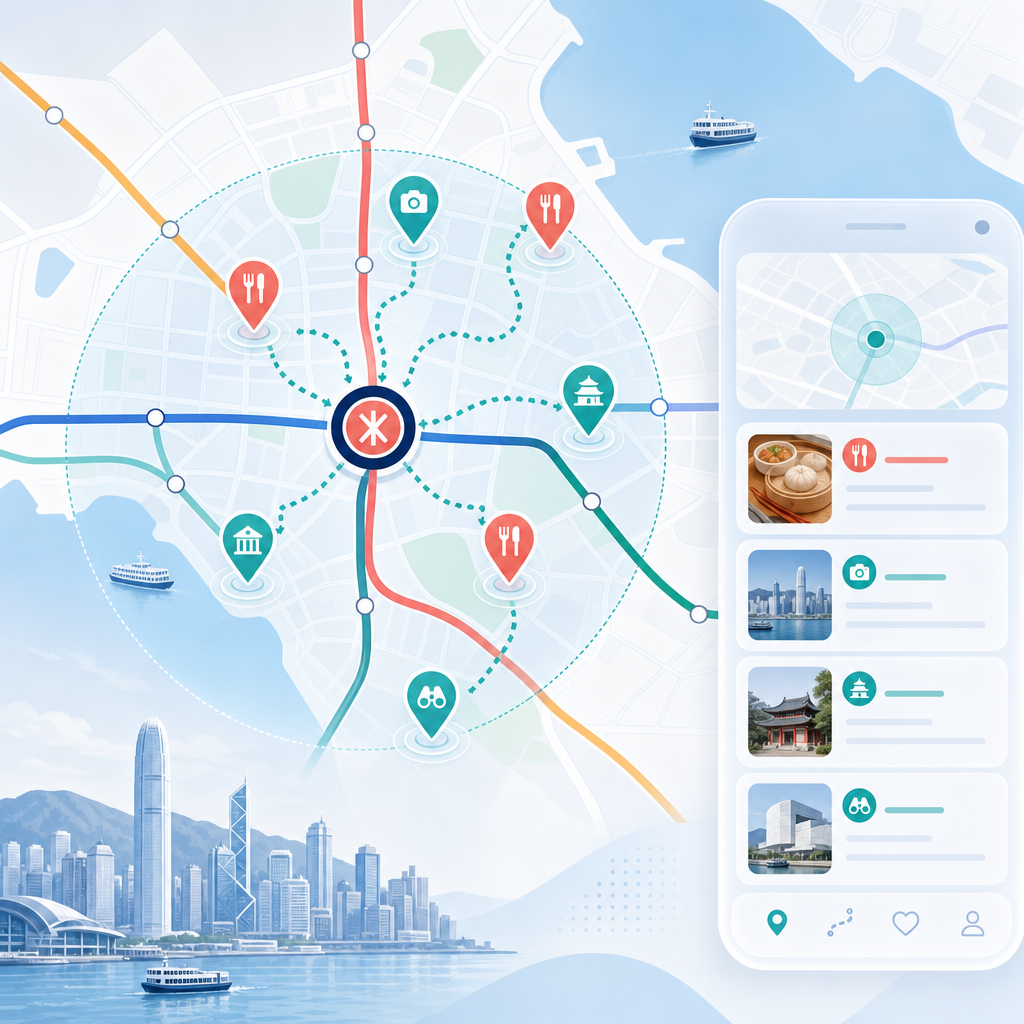
\includegraphics[width=\linewidth,height=4.35cm,keepaspectratio]{../assets/nearby-journey.png}};
        \node[anchor=south east,fill=white,fill opacity=0.92,text opacity=1,draw=linegray,
              rounded corners=4pt,inner xsep=6pt,inner ysep=3pt,font=\scriptsize]
          at (2.95,-2.10) {\textcolor{foodorange}{美食}\quad\textcolor{attrgreen}{景点}\quad\textcolor{accentred}{路线}};
      \end{tikzpicture}
    \end{column}
  \end{columns}

  \vskip3pt
  \begin{center}
  \begin{tikzpicture}[
    >=Stealth,
    pill/.style={rounded corners=7pt,line width=0.9pt,minimum width=3.05cm,minimum height=1.02cm,align=center,text=ink},
    arr/.style={-{Stealth[length=3mm]},line width=1.1pt,draw=linegray}]
    \node[pill,draw=mainblue,fill=mainblue!8] (a)
      {{\bfseries 呈现}\\[-1pt]{\scriptsize 卡片化，按需展开}};
    \node[pill,draw=foodorange,fill=foodorange!10,right=0.72cm of a] (b)
      {{\bfseries 决策}\\[-1pt]{\scriptsize 筛选、排序、推荐}};
    \node[pill,draw=attrgreen,fill=attrgreen!8,right=0.72cm of b] (c)
      {{\bfseries 探索}\\[-1pt]{\scriptsize 地图联动，串成路线}};
    \draw[arr] (a) -- (b);
    \draw[arr] (b) -- (c);
  \end{tikzpicture}
  \end{center}
\end{frame}

%==================== 第 2 页：卡片式呈现 + 渐进式披露 ====================
\begin{frame}{怎么看：卡片化呈现，按需展开}
  \begin{columns}[T,totalwidth=\textwidth]
    \begin{column}{0.33\textwidth}
      \footnotesize
      \begin{itemize}\setlength\itemsep{4pt}
        \item 卡片首层放判断线索：缩略图、名称、类型、距离、步行时间、价位与评分。
        \item 点开后再显示大图、简介、营业时间、定位、加入路线、电话与官网。
        \item 没有照片时，用稳定的菜系底图补位，列表不留空洞，滚动时也更稳定。
      \end{itemize}
    \end{column}
    \begin{column}{0.64\textwidth}
      \begin{minipage}[t]{0.30\linewidth}
        \centering
        \shot{0.97\linewidth}{4.65cm}{screenshots/lrg-4.png}\tightimgcap{卡片展开：摘要到详情}
      \end{minipage}\hfill
      \begin{minipage}[t]{0.66\linewidth}
        \centering
        \shottrim{0.97\linewidth}{4.65cm}{150}{260}{0}{0}{screenshots/lrg-7.png}\tightimgcap{站点弹窗与周边面板形成连续入口}
      \end{minipage}
    \end{column}
  \end{columns}
\end{frame}

%==================== 第 3 页：筛选 · 排序 · 推荐 ====================
\begin{frame}{怎么选：把上百个选择，收敛成几个}
  \begin{columns}[T]
    \begin{column}{0.34\textwidth}
      \footnotesize
      \begin{itemize}\setlength\itemsep{4pt}
        \item 分类、菜系、半径与排序集中在同一区域，操作路径更短。
        \item 推荐、距离、评分三种排序保留选择权；随机按钮缓解临时决策压力。
        \item 卡片持续显示距离、步行分钟、评分和来源，排序依据更容易判断。
        \item 筛空时给出扩大半径按钮，用户能直接恢复探索。
      \end{itemize}
    \end{column}
    \begin{column}{0.64\textwidth}
      \begin{minipage}[t]{0.29\linewidth}
        \centering
        \shot{\linewidth}{4.68cm}{screenshots/lrg-3.png}\tightimgcap{筛选控件集中}
      \end{minipage}\hfill
      \begin{minipage}[t]{0.67\linewidth}
        \centering
        \shottrim{\linewidth}{4.68cm}{740}{0}{0}{0}{screenshots/lrg-5.png}\tightimgcap{筛空后给出“扩大半径”的可执行出口}
      \end{minipage}
    \end{column}
  \end{columns}
\end{frame}

%==================== 第 4 页：地图联动 + 逛吃路线 ====================
\begin{frame}{怎么逛：地图联动，串成一条路线}
  \begin{columns}[T]
    \begin{column}{0.38\textwidth}
      \footnotesize
      \begin{itemize}\setlength\itemsep{3pt}
        \item 列表与地图双向联动：点卡片会定位，点标记会回到对应卡片。
        \item 菜系图标、颜色、半径圈和聚合点共同说明可达范围。
        \item 加入逛吃路线后，系统用虚线串联编号点，并计算总步行时长。
      \end{itemize}
    \end{column}
    \begin{column}{0.60\textwidth}
      \centering
      \shot{\linewidth}{2.66cm}{screenshots/lrg-1.png}\tightimgcap{半径圈、标记与面板联动}\\[1pt]
      \shot{\linewidth}{2.36cm}{screenshots/lrg-6.png}
    \end{column}
  \end{columns}
\end{frame}

%==================== 第 5 页：设计原因（一）信息组织与认知负荷 ====================
\begin{frame}{设计依据（一）：信息组织与认知负荷}
  \begin{columns}[T]
    \begin{column}{0.60\textwidth}
      \small
      \begin{itemize}\setlength\itemsep{4pt}
        \item \textbf{\color{mainblue}视觉感知与信息层级}：用户先扫图、名称、距离、评分；界面把这些线索放在卡片首层，细节留给展开层。
        \item \textbf{\color{mainblue}格式塔分组}：卡片边框、留白和统一排版把每个地点分成清晰对象；同类标签用相近样式，分类关系更容易被看出。
        \item \textbf{\color{mainblue}降低认知负荷}：分类、排序和半径滑块把大量兴趣点收进当前可比较范围，减少无关信息干扰，也回应了选择过多带来的犹豫。
        \item \textbf{\color{mainblue}识别代替记忆}：照片、菜系图标、距离和步行分钟都作为外部线索，用户根据界面判断，不需要记住站点周边情况。
      \end{itemize}
    \end{column}
    \begin{column}{0.38\textwidth}
      \centering
      \begin{tikzpicture}
        \node[inner sep=0pt,rounded corners=8pt,
              draw=linegray,line width=0.6pt,
              drop shadow={shadow xshift=0.6pt,shadow yshift=-0.8pt,opacity=0.16}]
          {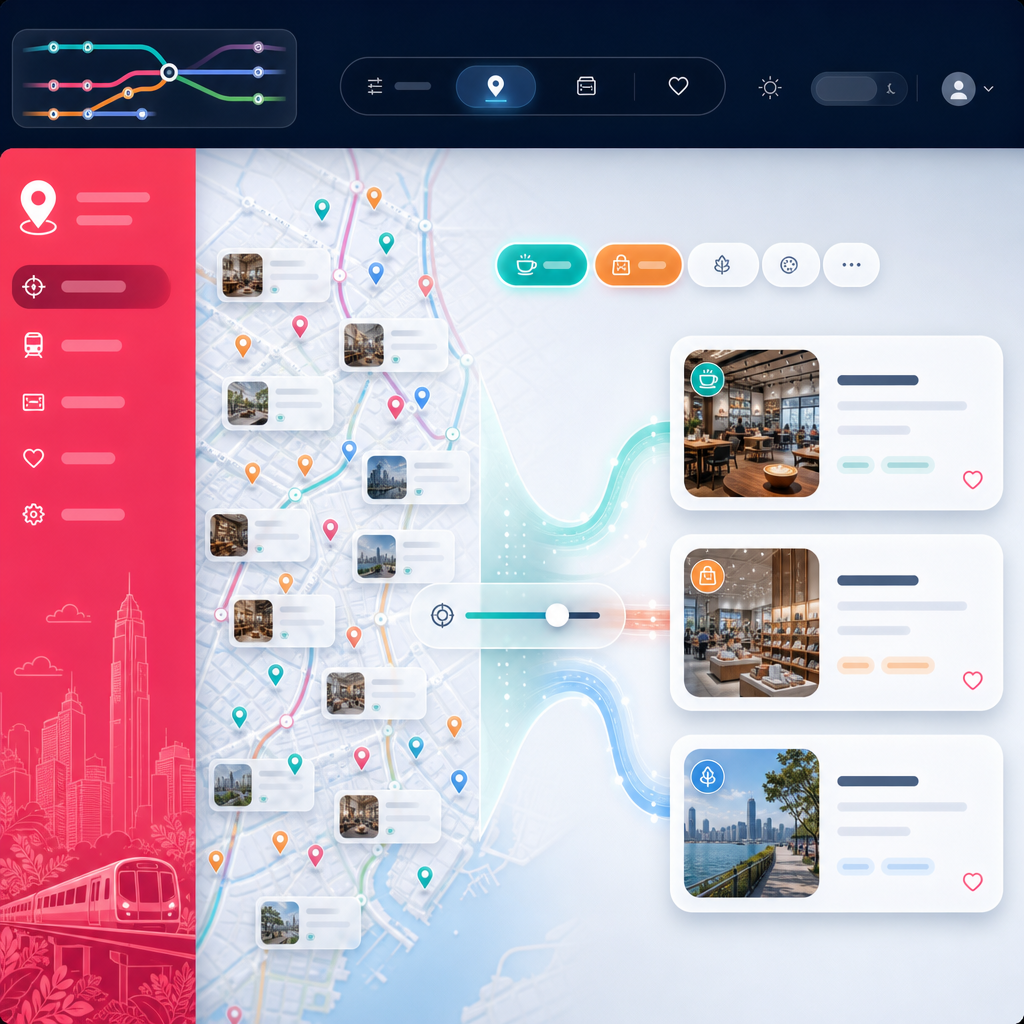
\includegraphics[width=\linewidth,height=4.10cm,keepaspectratio]{../assets/choice-funnel-v2.png}};
        \node[anchor=north west,fill=white,fill opacity=0.94,text opacity=1,draw=mainblue!20,
              rounded corners=4pt,inner xsep=5pt,inner ysep=2pt,font=\tiny\bfseries,text=ink]
          at (-2.10,2.05) {候选很多};
        \node[fill=mainblue,text=white,rounded corners=4pt,inner xsep=5pt,inner ysep=2pt,font=\tiny\bfseries]
          at (0.03,0.18) {筛选 / 排序 / 推荐};
        \node[anchor=south east,fill=mint,draw=attrgreen!28,rounded corners=4pt,
              inner xsep=5pt,inner ysep=2pt,font=\tiny\bfseries,text=ink]
          at (2.05,-2.03) {少量可行动选择};
      \end{tikzpicture}
      \tightimgcap{把选择成本一路收窄}
    \end{column}
  \end{columns}
\end{frame}

%==================== 第 6 页：设计原因（二）状态、反馈与用户控制 ====================
\begin{frame}{设计依据（二）：状态、反馈与用户控制}
  \begin{columns}[T]
    \begin{column}{0.58\textwidth}
      \small
      \begin{itemize}\setlength\itemsep{6pt}
        \item \textbf{\color{mainblue}系统状态可见}：当前站点、地点数量、排序方式、探索半径和地图标记持续可见，用户知道自己正在看哪一片区域。
        \item \textbf{\color{mainblue}反馈及时}：点击卡片、地图标记或加入路线后，地图与列表同步变化，操作结果留在同一上下文里。
        \item \textbf{\color{mainblue}防错与修正}：筛空时显示原因和扩大半径按钮，用户可以直接恢复探索。
        \item \textbf{\color{mainblue}用户控制}：系统给出推荐和路线建议，收藏、加入路线、扩大范围都由用户确认，探索节奏由用户掌握。
      \end{itemize}
    \end{column}
    \begin{column}{0.40\textwidth}
      \centering
      \shot{\linewidth}{3.34cm}{screenshots/lrg-2.png}
      \imgcap{真实界面：状态、筛选和地图反馈同时可见}
    \end{column}
  \end{columns}
\end{frame}

\end{document}
